\documentclass[
	12pt,				% tamanho da fonte
	openright,			% capítulos começam em pág ímpar (insere página vazia caso preciso)
	oneside,			% para impressão somente em um lado da folha.
%	twoside,			% para impressão em verso e anverso. Oposto a oneside
	a4paper,			% tamanho do papel. 
	% -- opções da classe abntex2 --
	chapter=TITLE,		% títulos de capítulos convertidos em letras maiúsculas
%	section=TITLE,		% títulos de seções convertidos em letras maiúsculas
	%subsection=TITLE,	% títulos de subseções convertidos em letras maiúsculas
	%subsubsection=TITLE,% títulos de subsubseções convertidos em letras maiúsculas
	% -- opções do pacote babel --
	english,			% idioma adicional para hifenização
	brazil				% o último idioma é o principal do documento
	]{abntex2temp} % classe abntex2ufop para escrita de trabalhos academicos

% ---
% Pacotes básicos 
% ---
\usepackage{float}
%\usepackage{lmodern}			% Usa a fonte Latin Modern	
\usepackage{times}				% Usa a fonte Latin Modern	
\usepackage{fancyvrb}			% Para mudança de fonte ambiente verbatim
\DefineVerbatimEnvironment{verbatim}{Verbatim}{fontfamily=zi4}
\usepackage[T1]{fontenc}		% Selecao de codigos de fonte.
\usepackage[utf8]{inputenc}		% Codificacao do documento (conversão automática dos acentos)

\usepackage{lastpage}			% Usado pela Ficha catalográfica
\usepackage{indentfirst}		% Indenta o primeiro parágrafo de cada seção.
\usepackage{color}				% Controle das cores
\usepackage{graphicx}			% Inclusão de gráficos
\usepackage{microtype} 			% para melhorias de justificação
\usepackage{supertabular}       % tabela na capa do documento
% ---
		
% ---
% Pacotes adicionais, usados apenas no âmbito do Modelo Canônico do abnteX2 - pode ser removido

% ---
% Pacotes adicionais, usados no anexo do modelo de folha de identificação
% ---
\usepackage{multicol}
\usepackage{multirow}
\usepackage{lipsum}				% para geração de dummy text
% ---
% Pacotes de citações
% ---
\usepackage[brazilian,hyperpageref]{backref}	 % Paginas com as citações na bibliografia
\usepackage[alf]{abntex2cite}	% Citações padrão ABNT 6023

% ----
\usepackage{amsmath} % mathematical features
\usepackage{amssymb}
% ----

% --- 
% CONFIGURAÇÕES DE PACOTES
% --- 

% ---
% Configurações do pacote backref
% Usado sem a opção hyperpageref de backref
\renewcommand{\backrefpagesname}{Citado na(s) página(s):~}
% Texto padrão antes do número das páginas
\renewcommand{\backref}{}
% Define os textos da citação
\renewcommand*{\backrefalt}[4]{
	\ifcase #1 %
		Nenhuma citação no texto.%
	\or
		Citado na página #2.%
	\else
		Citado #1 vezes nas páginas #2.%
	\fi}%
% ---

% ---
% Informações de dados para CAPA e FOLHA DE ROSTO
% ---
\titulo{Simulação de modelos epidemiológicos em redes de mobilidade temporais}
\autor{Gabriel Ferreira da Costa}
\local{Ouro Preto - Minas Gerais - Brasil}
\data{Setembro de 2023}
\orientador{Prof. Dr. Vander Luis de Souza Freitas}
\instituicao{Universidade Federal de Ouro Preto}
\unidade{Departamento de Computação}
\tipotrabalho{Relatório final do projeto de iniciação científica\\EDITAL 04/2022 PIBIC/CNPQ-2022/23\\Vigência: 01/09/2022 a 31/08/2023}
% O preambulo deve conter o tipo do trabalho, o objetivo, 
% o nome da instituição e a área de concentração 
%\preambulo{}
% ---


% ---
% Configurações de aparência do PDF final

% alterando o aspecto da cor azul
\definecolor{hexagram}{RGB}{2, 235, 239}
\definecolor{hexagram1}{RGB}{255, 0, 0}
\definecolor{hexagram2}{RGB}{106, 188, 68}
\definecolor{blue}{RGB}{41,5,195}

% informações do PDF
\makeatletter
\hypersetup{
     	%pagebackref=true,
		pdftitle={\@title}, 
		pdfauthor={\@author},
    	pdfsubject={\imprimirpreambulo},
	    pdfcreator={LaTeX with abnTeX2},
		pdfkeywords={abnt}{latex}{abntex}{abntex2}{trabalho acadêmico}, 
		colorlinks=true,       		% false: boxed links; true: colored links
    	linkcolor=blue,          	% color of internal links
    	citecolor=blue,        		% color of links to bibliography
    	filecolor=magenta,      		% color of file links
		urlcolor=blue,
		bookmarksdepth=4
}
\makeatother
% --- 

% --- 
% Espaçamentos entre linhas e parágrafos 
% --- 

% O tamanho do parágrafo é dado por:
\setlength{\parindent}{1.3cm}

% Controle do espaçamento entre um parágrafo e outro:
\setlength{\parskip}{0.2cm}  % tente também \onelineskip

% ---
% compila o indice
% ---
\makeindex
% ---

% ----
% Início do documento
% ----
\begin{document}
% Retira espaço extra obsoleto entre as frases.
\frenchspacing 
% ------------------------------------------
% ELEMENTOS PRÉ-TEXTUAIS
% ------------------------------------------
% \pretextual
% ---
% Capa
% ---
\imprimircapa
% ---
% ---
% Folha de rosto
% (o * indica que haverá a ficha bibliográfica)
% ---
%\imprimirfolhaderosto*
% ---
% RESUMOS
% ---
% resumo em português
\setlength{\absparsep}{18pt} % ajusta o espaçamento dos parágrafos do resumo
\begin{resumo}
 \noindent O presente projeto tem por objetivo simular modelos epidemiológicos em redes de mobilidade temporais. Busca-se comparar os resultados obtidos a partir de redes dinâmicas e versões estáticas. A segunda estratégia é comumente utilizada, partindo da agregação dos estados da rede em vários instantes de tempo, dentro de uma janela temporal - uma simplificação dos fluxos de pessoas entre localidades. Entretanto, ter disponível os estados da rede em diferentes instantes de tempo é útil para a obtenção de resultados parciais mais fidedignos, isto é, números de casos confirmados, pessoas infectadas, mortes, etc., mais acurados durante a simulação. Alguns pontos que serão investigados no presente projeto são: a quantificação das diferenças entre a dinâmica simulada na rede temporal e sua versão estática; qual a tolerância na alteração da escala temporal da rede em relação à sua versão mais refinada, ou seja, verificar se é possível agregar alguns estados da rede e ainda assim obter os mesmo resultados e; investigar as correspondências entre as mudanças na dinâmica com as mudanças topológicas da rede, no tempo.

 \textbf{Palavras-chave}: Redes complexas, redes de mobilidade, redes temporais, redes dinâmicas, epidemiologia.
\end{resumo}

%O uso de séries temporais está presente em diversas áreas da ciência, sejam elas naturais, humanas, exatas ou biológicas. A análise dessas séries, portanto, se faz necessária, assim como o desenvolvimento de diversas ferramentas para tal propósito. Modelos matemáticos e estatísticos estão sempre presentes na representação da dinâmica de uma série temporal, mas novas abordagens estão obtendo êxito nesse fim. A incorporação da teoria dos grafos na análise da dinâmica de séries temporais vem sendo usada recentemente na literatura; séries são convertidas em redes compostas por nós e arestas, que por sua vez são analisadas usando o ferramental presente no estudo dos grafos.

% resumo em inglês
%\begin{resumo}[Abstract]
% \begin{otherlanguage*}{english}

%\noindent This is the english abstract.

%   \vspace{\onelineskip}
 
%   \noindent 
%   \textbf{Key-words}: word1. word2. word3.
% \end{otherlanguage*}
%\end{resumo}

% ---
% inserir lista de figuras
% ---
%\pdfbookmark[0]{\listfigurename}{lof}
%\listoffigures*
%\cleardoublepage
% ---

% ---
% inserir lista de tabelas
% ---
%\pdfbookmark[0]{\listtablename}{lot}
%\listoftables*
%\cleardoublepage
% ---

% ---
% inserir lista de abreviaturas e siglas
% ---
%\begin{siglas}
%  \item[ABNT] Associação Brasileira de Normas %Técnicas
%  \item[abnTeX] ABsurdas Normas para TeX
%\end{siglas}
% ---

% ---
% inserir lista de símbolos
% ---
%\begin{simbolos}
%  \item[$ \Gamma $] Letra grega Gama
%  \item[$ \Lambda $] Lambda
%  \item[$ \zeta $] Letra grega minúscula zeta
%  \item[$ \in $] Pertence
%\end{simbolos}
% ---

% ---
% inserir o sumario
% ---
\pdfbookmark[0]{\contentsname}{toc}
\tableofcontents*
\cleardoublepage
% ---

% ------------------------------------------
% ELEMENTOS TEXTUAIS
% ------------------------------------------
\textual
\pagestyle{simple}

% ---
% Capítulos
% ---
\chapter[Introdução]{Introdução}
Uma rede complexa é um grafo composto por vértices, representando entidades que compõem o sistema complexo em estudo, e arestas, as quais capturam as interações entre eles. Exemplos são redes de mobilidade, a Internet e redes sociais \cite{BOCCALETTI2006, barabasi2016network}.

Uma importante característica de redes reais é sua evolução no tempo \cite{Kim2012, Masuda2021}. Há diversas formas de representação de redes temporais, como as redes agregadas e os grafos de eventos, transmissão, alcançabilidade e afins \cite{Sano2021}. Métricas comuns, como grau e betweenness, devem ser adaptadas a depender do tipo de representação, pois as noções de conectividade e caminho mínimo são, nesses casos, atreladas ao tempo. 

Redes de mobilidade são caracterizadas por nós que representam localidades e links que denotam o fluxo de pessoas entre um nó e outro, em uma dada janela de tempo \cite{Lamosa2021}. No caso específico dessas redes, algumas bases de dados disponibilizam dados estáticos com uma ou mais camadas \cite{Cavararo2017, 50OD} e outras com camadas e componente temporal \cite{Gallotti_2015}. Processos epidemiológicos, por exemplo, podem ser simulados com
maior riqueza de detalhes quanto mais completa for a representação da rede. 

Este projeto busca investigar: a quantificação das diferenças entre a dinâmica simulada na rede temporal e sua versão estática; qual a tolerância na alteração da escala temporal da rede em relação à sua versão mais refinada, ou seja, verificar se é possível agregar alguns estados da rede e ainda assim obter os mesmo resultados e; as correspondências entre as mudanças na dinâmica com as mudanças topológicas da rede, no tempo. Neste projeto, foi utilizado o modelo compartimental SIR, com metapopulações \cite{Kermack1927, Harko2014}, para simulação de epidemias.


\chapter{Objetivos}
%Dentro dos objetivos compreendidos como gerais, busca-se apresentar os resultados obtidos durante o período de duração do projeto. 
%Os objetivos específicos são apresentados a seguir:
%\begin{itemize}
%\item Explorar e comparar os algoritmos usados para conversão de séries temporais %em redes complexas;
%\item Estudar sistemas com base na análise de suas representações como redes %complexas.
%\end{itemize}

O objetivo geral é investigar a dinâmica de processos epidemiológicos em redes de mobilidade temporais e compará-la com a dinâmica em redes de mobilidade estáticas.

Os objetivos específicos são:

\begin{itemize}
    \item Realizar uma revisão de literatura sobre os métodos utilizados para resolver o problema
    abordado.
    \item Modelar processos epidemiológicos em redes de mobilidade.
    \item Simular os processos em redes temporais em diferentes escalas de tempo.
    \item Simular os processos em redes estáticas e comparar com o caso temporal.
    \item Contribuir com a divulgação de técnicas aplicadas à resolução do problema.
    \item Colaborar com a formação de recursos humanos especializados nesta área do
    conhecimento.
    \item Favorecer a consolidação do Laboratório de Computação de Sistemas Inteligentes
    (CSILab) da Universidade Federal de Ouro Preto.
\end{itemize}

\chapter{Revisão da literatura}

\section{Redes complexas e grafos}

Estamos rodeados por sistemas irremediavelmente complexos que envolvem interações em grande escala. Exemplos disso incluem sociedades com bilhões de indivíduos cooperando, infraestruturas de comunicação conectando milhões de telemóveis, computadores e satélites, e a atividade coordenada de bilhões de neurônios em nosso cérebro para compreender o mundo. Além disso, nossa biologia depende de inúmeras interações entre genes e metabolitos nas células \cite{Albert_2002}.

Esses sistemas são chamados coletivamente de sistemas complexos devido à dificuldade em prever seu comportamento com base no conhecimento de seus componentes individuais. Dada a importância desses sistemas em nossa vida cotidiana, na ciência e na economia, compreender, descrever matematicamente, prever e até controlar sistemas complexos se tornou um dos principais desafios intelectuais e científicos do século XXI.

Um recurso fundamental para abordar essa complexidade é a teoria dos grafos, que representa sistemas como conjuntos de nós interconectados por arestas. As redes são uma poderosa abordagem para estudar sistemas complexos em diversas áreas, como biologia, sociologia, tecnologia e transporte \cite{barabasi2016network}.

\begin{figure}[!h]
    \centering
    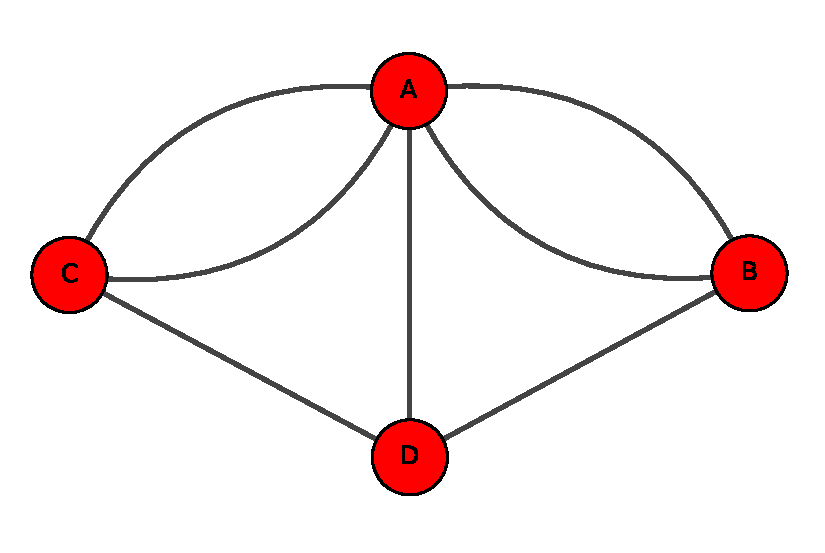
\includegraphics[width=8cm]{figures/konigsberg.pdf}
    \caption{A figura apresenta o grafo que descreve a solução do famoso problema das sete pontes de Königsberg. Este desafio histórico, resolvido por \citeonline{Euler1736}, originou a teoria dos grafos.}
    \label{fig:basin-region}
\end{figure}

Os links de uma rede podem ser direcionados ou não direcionados, e essa distinção desempenha um papel crucial na modelagem de sistemas complexos. Redes com links direcionados, como a World Wide Web (WWW) ou chamadas telefônicas, têm conexões unilaterais, onde a direção importa, indicando que um nó está conectado a outro de forma diferente da recíproca. Por outro lado, redes não direcionadas, como relacionamentos ou linhas de transmissão elétrica, refletem conexões bidirecionais, onde a relação é simétrica. Além disso, algumas redes combinam ambos os tipos de conexões, como as redes metabólicas, onde algumas reações são reversíveis (bidirecionais) e outras são irreversíveis (direcionadas).

A representação matemática de uma rede é essencial para sua análise. Uma rede é formalmente definida como um grafo $G(V, E)$, onde $V$ representa os nós (ou vértices) da rede e $E$ representa as arestas (ou links) entre esses nós. Dentro deste contexto, muitas vezes trabalhamos com redes ponderadas, onde os pesos das arestas ($W_{ij}$) entre pares de nós ($i$ e $j$) representam valores como fluxos, distâncias ou outras medidas relevantes para o sistema. Essa abordagem matemática permite a aplicação de técnicas de análise de grafos para entender a topologia e dinâmica das redes complexas que permeiam nosso mundo \cite{Newman2010}.

Uma descrição completa de uma rede exige que acompanhemos seus links. A maneira mais simples de conseguir isso é fornecer uma lista completa dos links \cite{barabasi2016network}. Para fins matemáticos, frequentemente representamos uma rede através de sua matriz de adjacência. A matriz de adjacência de uma rede direcionada de $N$ nós possui $N$ linhas e $N$ colunas, sendo seus elementos:
\begin{align*}
    A_{ij} =
    \begin{cases}
        1, & \text{se existe um link apontando do nó } j \text{ para o nó } i \\
        0, & \text{se os nós } i \text{ e } j \text{ não estiverem conectados entre si}
    \end{cases}
\end{align*}

A matriz de adjacência de uma rede não direcionada possui duas entradas para cada link, por ex. o link (1, 2) é representado como $A_{12} = 1$ e $A_{21} = 1$. Portanto, a matriz de adjacência de uma rede não direcionada é simétrica, $A_{ij} = A_{ji}$.

A matriz de adjacência desempenha um papel fundamental na análise de redes, pois permite representar de forma clara e concisa a conectividade entre os nós. Ela é especialmente útil para calcular propriedades como o grau dos nós, identificar subgrafos e realizar diversas análises matemáticas e estatísticas sobre a rede. Além disso, a matriz de adjacência pode ser empregada em algoritmos que exploram a estrutura da rede para resolver uma variedade de problemas, desde encontrar caminhos mais curtos até identificar comunidades de nós.

Portanto, a matriz de adjacência desempenha um papel central na análise e modelagem de redes complexas, permitindo-nos explorar e compreender as interações entre seus componentes.

\section{Redes temporais}

A compreensão de sistemas complexos, sejam eles biológicos, sociais ou tecnológicos, muitas vezes exige uma perspectiva de longo alcance que nos permita observar a organização global e suas interações fundamentais. A modelagem de redes oferece uma abordagem valiosa para simplificar a complexidade, concentrando-se nas unidades e conexões que compõem esses sistemas. No entanto, uma dimensão crucial muitas vezes negligenciada é o tempo. 

A rede temporal, uma extensão da modelagem de redes, aborda essa lacuna ao não apenas considerar quais unidades estão interconectadas, mas também quando essas interações ocorrem. Essa abordagem não se limita apenas a sistemas biológicos ou sociais, mas abrange uma ampla gama de contextos, desde infraestruturas tecnológicas até interações ecológicas. Ao incorporar o fator temporal, as redes temporais nos capacitam a capturar nuances e dinâmicas que podem ser essenciais para uma compreensão completa dos sistemas em estudo \cite{HOLME201297}.

As redes dinâmicas, aquelas que evoluem ao longo do tempo, desempenham um papel de destaque na compreensão dos processos de disseminação, abrangendo desde a propagação de informações até a disseminação de doenças \cite{HOLME201297}. Isso se deve ao fato de que, em tais redes, cada conexão entre elementos representa uma oportunidade de interação, e a sequência temporal dessas interações é cuidadosamente registrada.

As escalas de tempo, representadas por $t_N$ e $t_P$, desempenham um papel fundamental na análise de redes temporais. O valor de $t_N$ refere-se à escala de tempo característica para a evolução da própria rede, ou seja, quanto tempo leva para que a estrutura da rede se modifique de maneira significativa. Por outro lado, $t_P$ representa a escala de tempo característica para a dinâmica do processo de propagação que ocorre sobre essa rede.

Em cenários onde $t_N$ é consideravelmente maior do que $t_P$ (ou seja, $t_N \gg t_P$), a rede evolui em um ritmo relativamente lento em comparação com a dinâmica do processo, tornando possível uma abordagem estática da rede para simplificar a modelagem do fenômeno em questão. No entanto, quando $t_N$ e $t_P$ são da mesma ordem de grandeza (ou seja, $t_N \sim t_P$), as redes temporais se destacam, pois a interação entre a evolução da rede e o processo de propagação torna-se significativa e não pode ser negligenciada. Por fim, em cenários onde a rede evolui rapidamente em relação ao processo (ou seja, $t_N \ll t_P$), pode ser apropriado usar uma abordagem de rede média no tempo para simplificar a modelagem.

Essa distinção entre as escalas de tempo nos permite escolher a abordagem mais adequada para cada situação, adaptando-a à natureza e à temporalidade dos processos em sistemas complexos.

\section{Modelos epidemiológicos}

A modelagem em epidemiologia compartilha objetivos similares com a modelagem ecológica, centrando-se na compreensão da prevalência, distribuição e fatores que influenciam a incidência, propagação e persistência de doenças. Enquanto na ecologia, a quantificação precisa da abundância de espécies frequentemente é de grande interesse, na epidemiologia, o foco recai na categorização dos indivíduos de acordo com seu estado de infecção em uma população hospedeira \cite{Matt2008}. Nesse contexto, os modelos epidemiológicos podem ser comparados aos modelos de metapopulação da ecologia \cite{macarthur1967theory, levins1969demographic}, onde cada indivíduo é considerado como um recurso para o patógeno, com processos de transmissão e recuperação análogos à dispersão e extinção. A modelagem matemática em epidemiologia tem uma longa história e tem sido aplicada desde o século XVIII, passando por desenvolvimentos conceituais e técnicos significativos.

A modelagem de epidemias envolve duas abordagens principais: estocástica e determinística.

Nos modelos estocásticos, a aleatoriedade está presente nas variáveis, permitindo estimar distribuições de probabilidade de resultados possíveis, especialmente quando as flutuações aleatórias têm um papel significativo, como em populações pequenas ou em cenários com variações casuais marcantes.

Por outro lado, os modelos determinísticos são empregados para grandes populações, como por exemplo para o estudo da tuberculose. Neles, a população é dividida em compartimentos representando diferentes estágios da epidemia. As taxas de transição entre esses compartimentos são descritas por equações diferenciais.

Além disso, é importante destacar que, ao longo deste estudo, trabalharemos com a suposição de que a população em análise apresenta uma mistura homogênea, ou seja, todos os indivíduos interagem igualmente entre si \cite{allman_rhodes_2003}. Essa premissa implica que o risco de exposição à doença por parte dos não infectados é uniforme em relação aos indivíduos já infectados.

\subsection{Modelo SIR}

O modelo epidêmico mais simples, porém poderoso, que podemos considerar é o modelo SIR. Neste, os membros da população progridem através de três compartimentos, da seguinte forma:
\begin{itemize}
    \item \textcolor{hexagram}{\textbf{Suscetíveis (S)}}: Esta classe representa os indivíduos que estão em risco de contrair a doença, mas que atualmente não estão infectados.
    \item \textcolor{hexagram1}{\textbf{Infectados (I)}}: Aqui, encontramos aqueles que já foram infectados pela doença e são atualmente contagiosos.
    \item \textcolor{hexagram2}{\textbf{Removidos (R)}}: Esta classe abrange os indivíduos que não podem mais contrair a doença, seja porque se recuperaram completamente, desenvolveram imunidade natural ou, infelizmente, faleceram.
\end{itemize}

\begin{figure}[!h]
    \centering
    
\includegraphics[width=8cm]{figures/SIRmodel.png}
    \caption{Diagrama esquemático do modelo SIR, adaptado de \citeonline{barabasi2016network}.}
    \label{fig:SIR}
\end{figure}

A evolução de uma epidemia, como a da gripe, muitas vezes ocorre em um ritmo muito mais acelerado em comparação com as mudanças na taxa de natalidade e mortalidade. Como resultado, modelos compartimentais simplificados frequentemente excluem considerações sobre nascimentos e mortes, um aspecto conhecido como dinâmica vital (ou demografia). O sistema SIR sem a influência da dinâmica vital, para uma população com $N$ hospedeiros, pode ser representado por meio do seguinte conjunto de equações diferenciais ordinárias \cite{Hethcote2000}:
{\large
\begin{align}
\label{eq:sistema_equacoes}
\begin{cases}
\frac{dS}{dt} = -\frac{{\boldsymbol{\beta}} S I}{N}, \\
\frac{dI}{dt} = \frac{{\boldsymbol{\beta}} S I}{N} - \gamma I, \\
\frac{dR}{dt} = \gamma I.
\end{cases}
\end{align}}

Apesar de sua não linearidade, este sistema possibilita uma solução analítica implícita \cite{Harko2014}. Inicialmente, observe a seguinte relação:

{\large
\begin{equation}\label{eq:conservacao_populacao}
\frac{dS}{dt} + \frac{dI}{dt} + \frac{dR}{dt} = 0
\end{equation}}
Pode-se deduzir que:
{\large
\begin{equation}\label{eq:conservacao_populacao2}
S(t) + I(t) + R(t) = \text{constante} = N
\end{equation}}
A invariabilidade da população $N$ simplifica a análise, permitindo a consideração de apenas duas das três variáveis em questão.

A taxa de transmissão, $\beta$, é uma medida da probabilidade de um indivíduo infectado transmitir a doença a um indivíduo suscetível. Por exemplo, se $\beta$ for $0.1$, então um indivíduo infectado tem $10$\% de probabilidade de transmitir a doença a um indivíduo suscetível, ao entrar em contato com o mesmo, em um determinado período de tempo.

A taxa de recuperação, $\gamma$, é uma medida da rapidez com que um indivíduo infectado se recupera da doença. Por exemplo, se $\gamma$ for $0.2$, então um indivíduo infectado se recuperará da doença dentro de $5$ dias.

As unidades $\beta$ e $\gamma$ são importantes porque determinam o comportamento do modelo SIR. Se $\beta$ for maior que $\gamma$, então a doença se espalhará pela população. Se $\beta$ for menor que $\gamma$, a doença desaparecerá.

Em conjunto, esses dois parâmetros do modelo nos fornecem o \textit{número básico de  reprodução} $R_{0}$: uma medida representativa do número médio de infecções secundárias originadas a partir de um hospedeiro já infectado.

{\large
\begin{equation}
R_0 = \frac{\beta}{\gamma}
\label{eq:R0}
\end{equation}}

No cenário onde o valor de $R_{0}$ ultrapassa a marca de um, a taxa de infecção supera a taxa de recuperação, o que resulta no crescimento da infecção em toda a população. Por outro lado, quando $R_{0}$ permanece abaixo de um, a infecção tende a desaparecer rapidamente, uma vez que as pessoas se recuperam mais rapidamente do que contribuem para a propagação da doença.
\chapter{Trabalhos relacionados}

Neste capítulo, faremos um levantamento de trabalhos que aplicaram modelos epidemiológicos em diversas redes, abrangendo diferentes contextos, como a propagação de doenças infecciosas e informações em sistemas complexos. Para cada trabalho revisado, destacaremos os modelos utilizados, as características das redes e os resultados obtidos. Nosso objetivo é oferecer uma visão ampla das contribuições recentes no campo da epidemiologia de redes e como essas pesquisas têm contribuído para entender e prever processos de propagação em sistemas complexos.

\section{Signal propagation in complex networks}

A pesquisa conduzida por \citeonline{JI20231} é uma contribuição notável e extremamente relevante, abrangendo diversos modelos e redes complexas. Explora modelos fundamentais, como os epidêmicos, de Kuramoto, passeios aleatórios, reação-difusão e percolação, que descrevem a dinâmica de hospedeiros ou patógenos em redes de contato e a propagação de sinais. Além disso, investiga fatores topológicos, como redes temporais e multicamadas, e apresenta um quadro teórico abrangente para entender a interação entre dinâmica e topologia, destacando estudos recentes sobre o controle de redes.

O trabalho também se aprofunda em técnicas contemporâneas para analisar a propagação de sinais a partir de dados observacionais, abrangendo transferência de informações, métodos de inteligência artificial e análise de séries temporais em redes. Isso engloba a reconstrução da estrutura da rede, a localização das fontes de sinais e a previsão dos links entre os nós da rede. Além disso, aborda a análise de séries temporais impulsionada por IA, usando técnicas de aprendizado de máquina para processar e prever essas séries temporais.

Por fim, a pesquisa destaca aplicações significativas em campos como epidemias, dinâmica social, neurociência, redes de transmissão elétrica e robótica. Essas aplicações evidenciam a relevância das técnicas e modelos apresentados para compreender a propagação de doenças, a disseminação de informações em redes sociais e a confiabilidade das redes de comunicação. Em síntese, o trabalho de \citeonline{JI20231} proporciona uma visão abrangente e valiosa da dinâmica de propagação de sinais em redes complexas.

\section{Small but slow world: how network topology and burstiness slow down spreading}

\citeonline{Karsai_2011} conduziram um estudo que se baseou em dados empíricos de sequências de contatos, utilizando o modelo SI para analisar a dinâmica temporal da propagação de informações em redes de comunicação, com dados provenientes do conjunto de dados \textit{Reality Mining} \cite{Eagle2006}. Eles aplicaram modelos nulos para discernir os fatores que afetam essa propagação, destacando as correlações entre peso e topologia, bem como os padrões de atividade dos indivíduos como principais influências na desaceleração da propagação. O estudo também comparou redes de chamadas móveis e registros de e-mails, identificando diferenças notáveis. Por exemplo, na rede de chamadas móveis, chamadas consecutivas para muitas pessoas em curtos períodos impulsionaram um aumento acentuado na prevalência, enquanto na rede de e-mails, hubs com alto grau de comunicação desempenharam um papel fundamental na rápida propagação. Além disso, a pesquisa explorou como os padrões diários de atividade afetam a dinâmica de propagação, considerando os pesos das conexões. Em resumo, o estudo proporciona valiosas perspectivas sobre como a topologia e a intermitência da rede podem influenciar a velocidade de propagação nas redes de comunicação.

\section{Networks and epidemic models}

Outro trabalho que foi de grande valia para o desenvolvimento de nossa pesquisa foi conduzido por \citeonline{keeling2005networks}. Foi realizado um estudo abrangente na área da epidemiologia de doenças infecciosas, explorando uma ampla gama de modelos e estruturas de redes. Os modelos investigados incluíram aproximações em pares, modelos compartimentais (como SIR e SEIR), modelos baseados em agentes e modelos estocásticos. Além disso, diferentes tipos de redes foram analisados, desde redes de mistura completa até redes aleatórias, sem escala e de mundo pequeno, incluindo também redes de contato e árvores de transmissão.

Vale ressaltar que essa lista não é exaustiva, visto que a escolha de modelos e redes depende dos objetivos específicos de cada estudo e dos dados disponíveis. Esta pesquisa enfatiza a aplicação de modelos matemáticos na simulação da propagação de doenças infecciosas em redes de contatos individuais, fornecendo insights cruciais para a previsão da dinâmica epidêmica, a avaliação de estratégias de intervenção e a identificação de fatores determinantes na transmissão de doenças.

Ademais, essa investigação destaca a importância de selecionar a estrutura de rede mais adequada às características do problema e aos dados disponíveis, seja ela uma rede de mistura completa, aleatória, sem escala ou outra. Os resultados obtidos por meio desses modelos baseados em redes têm contribuído de forma substancial para a compreensão dos padrões de transmissão de doenças e o desenvolvimento de estratégias eficazes de controle, incluindo a identificação de indivíduos denominados \textit{superpropagadores} e a avaliação do impacto de campanhas de vacinação direcionadas.

\section{Comparing metapopulation dynamics of infectious diseases under different models of human movement}

O trabalho do qual obtivemos modelos fundamentais para o progresso de nosso projeto é o de \citeonline{Citron2021}. Neste estudo, são discutidos modelos de metapopulações compartimentais que incorporam o movimento dos hospedeiros e a dinâmica das doenças infecciosas. Os autores empregaram três modelos de transmissão de doenças infecciosas: o modelo suscetível-infectado-recuperado (SIR), o modelo suscetível-infectado-suscetível (SIS) \cite{Kermack1927} e o modelo Ross-Macdonald \cite{SIMOY2020105452}.

O modelo SIS divide a população em dois compartimentos, suscetíveis e infectados, com a possibilidade de indivíduos transitar entre esses estados. O modelo Ross-Macdonald, mais complexo, inclui a transmissão de doenças infecciosas por vetores.

Embora esta investigação não se concentre especificamente na malária, ela menciona um estudo de caso relacionado à transmissão e importação de malária na Ilha de Bioko, na Guiné Equatorial \cite{Guerra2019}. Neste contexto, os autores destacam a importância de selecionar modelos de movimento adequados. Eles utilizaram dados de inquéritos de indicadores da malária (MIS) \cite{citron2020supporting} para mapear a prevalência estimada da malária e a probabilidade estimada de um residente deixar a ilha . A análise mostrou uma taxa de risco elevada de infecção entre pessoas que relataram viagens recentes.

O estudo aplicou o modelo Ross-Macdonald para estimar o $R_{0}$ local, usando dados de prevalência e comportamento de viagem. Dados populacionais e estimativas geoespaciais foram essenciais para determinar a prevalência em cada local. Além disso, foram utilizados os destinos de viagem que as pessoas relataram para aprimorar um modelo que analisa como escolhem seus destinos ao viajar. Em resumo, esta pesquisa destaca a importância de modelar com precisão a mobilidade humana no controle de doenças infecciosas, com ênfase na malária na Ilha de Bioko.
\chapter{Metodologia}

A pergunta de pesquisa deste estudo investiga a dinâmica de processos epidemiológicos em redes de mobilidade temporais, em comparação com redes de mobilidade estáticas, com ênfase na variação da resolução temporal, ou seja, na granularidade da rede \cite{Pedrycz2002}. A metodologia envolve a variação da resolução temporal, desde uma rede por dia (melhor resolução - \textit{baseline}) até resoluções piores, como uma rede a cada 2 ou 3 dias. Observaremos o modelo \textit{SIR Euleriano} para compreender o impacto das diferentes escalas de tempo na propagação da doença. Posteriormente, compararemos os resultados obtidos em diferentes resoluções com o resultado da melhor resolução, utilizando alguma norma. Essa comparação é fundamental para avaliar a acurácia das modelagens em diferentes escalas de tempo e, assim, aprimorar as estratégias de controle epidemiológico.

\section{Metapopulações}

As metapopulações são um conceito fundamental em ecologia que descrevem grupos de populações de uma mesma espécie ocupando diferentes áreas geograficamente separadas e interagindo em algum nível. Esse termo foi cunhado por \citeonline{levins1969demographic} quando desenvolveu um modelo para entender a dinâmica populacional de pragas de insetos em campos agrícolas. No entanto, esse conceito tem sido amplamente aplicado em ecologia para compreender como as espécies respondem a ambientes fragmentados, sejam eles fragmentados naturalmente, como ocorre em ilhas, ou como resultado de ações humanas, como a destruição de habitats naturais.

Uma metapopulação consiste em várias populações distintas que ocupam áreas de habitat adequadas, incluindo algumas áreas ocasionalmente desocupadas. Cada população interage relativamente de forma independente com as outras e está sujeita a eventos demográficos aleatórios que podem levar à extinção local. À medida que as populações diminuem, aumenta o risco de desaparecimento devido a fatores diversos. No entanto, a metapopulação como um todo é mais estável, pois indivíduos de populações bem-sucedidas frequentemente migram para áreas desocupadas devido à extinção de outras populações, um processo chamado \textit{efeito de resgate}, crucial para a manutenção da metapopulação como um todo.

\begin{figure}[!h]
    \centering
    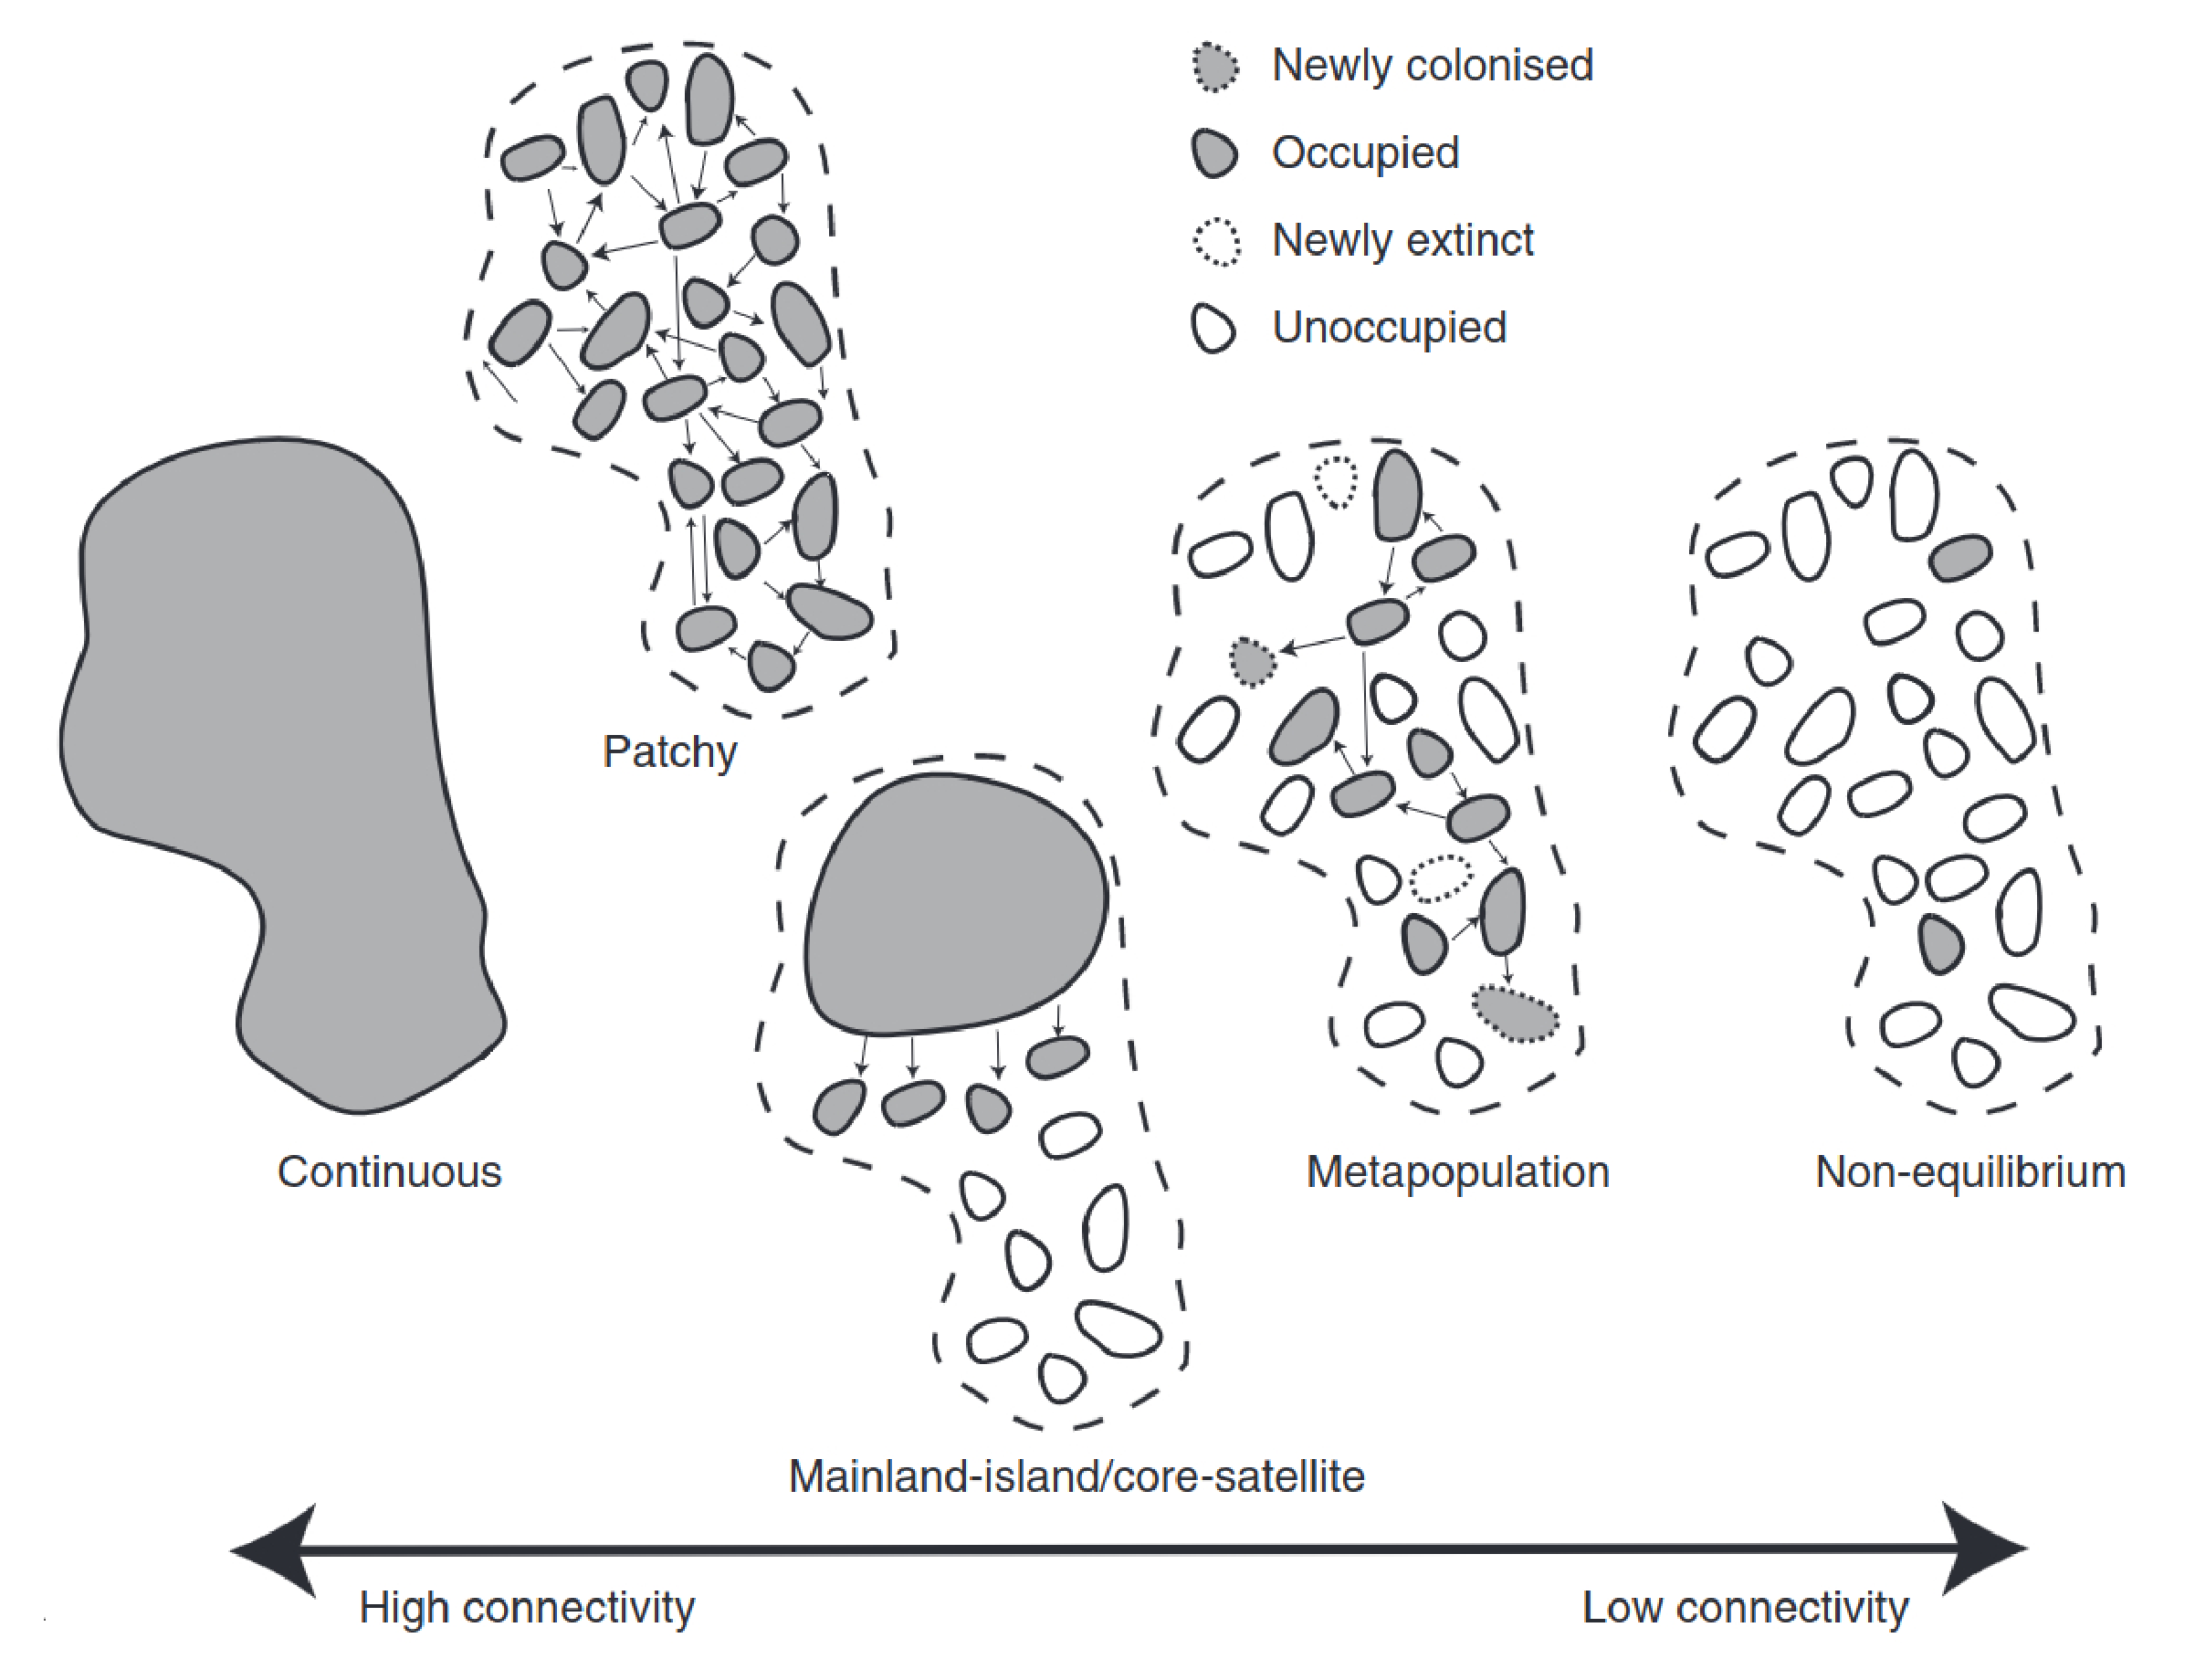
\includegraphics[width=10.8cm]{figures/metapop.pdf}
    \caption{Quatro tipos de modelos de metapopulação \cite{Harrison2008} com diferentes níveis de conectividade, adaptado de \citeonline{Nouhuys2009}.}
    \label{fig:metapopulations}
\end{figure}

\newpage

O termo \textit{subpopulações} é frequentemente usado de forma sinônima com \textit{populações locais} em contextos de metapopulação \cite{HanskiGaggiotti2004}. Estas subpopulações ou populações locais são grupos de indivíduos de uma espécie que ocupam áreas específicas dentro da metapopulação maior e estão interligados por meio de movimento entre essas áreas. Elas desempenham um papel fundamental na dinâmica da metapopulação, influenciando a sobrevivência e a distribuição da espécie em todo o conjunto de áreas ocupadas.

A fusão de redes e modelos epidemiológicos aos modelos de metapopulação oferece uma perspectiva mais abrangente para a compreensão da propagação de doenças infecciosas em sistemas complexos. As metapopulações podem ser pensadas como nós de uma rede complexa de manchas (\textit{patchies} em inglês) espaciais, onde os links codificam os fluxos humanos de um lugar para outro e são responsáveis pela transmissão entre manchas \cite{HAGENAARS2004349}, reforçando a importância da abordagem integrada. Esses modelos de metapopulação fornecem a estrutura básica para analisar a interação entre hospedeiros em diferentes áreas, presumindo uma mistura homogênea e contatos aleatórios localmente, o que permite uma visão geral das populações ao longo do tempo, calibrada com dados censitários.

No contexto de nosso projeto, incorporamos esses conceitos para entender a dinâmica de transmissão de doenças infecciosas em uma escala mais ampla. Ao combinar modelos de metapopulação com modelos epidemiológicos, podemos examinar como a transmissão de doenças ocorre localmente, levando em consideração a mobilidade das espécies hospedeiras. Essa abordagem é fundamental para entender os mecanismos de propagação de doenças infecciosas em nosso sistema e desenvolver estratégias eficazes de prevenção e controle, especialmente em sistemas complexos onde a conectividade entre populações desempenha um papel crucial.

\begin{figure}[!h]
    \centering
    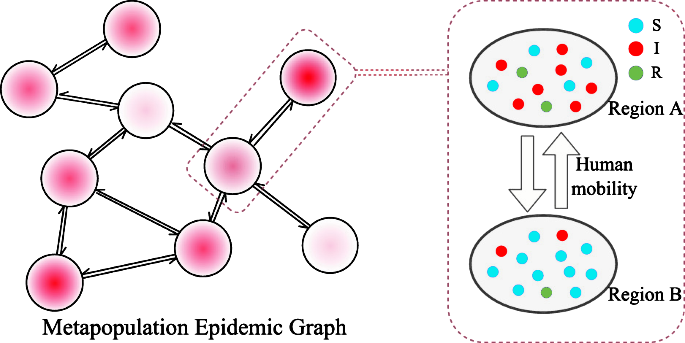
\includegraphics[width=10.8cm]{figures/metapopSIR.png}
    \caption{Modelo SIR em uma rede metapopulacional de manchas, adaptado de \citeonline{Cao2023}.}
    \label{fig:metapopulations}
\end{figure}

\newpage

\section{Modelos de movimento de hospedeiro}

Modelos de movimentação de hospedeiros, como os Eulerianos e Lagrangianos, são essenciais para simular a movimentação dentro de redes metapopulacionais. Enquanto os Eulerianos não rastreiam o comportamento individual e são adequados para descrever a migração animal, os Lagrangianos seguem os indivíduos e são mais adequados para descrever o comportamento de deslocamento humano \cite{Citron2021}.

Para compreender a difusão geográfica das doenças em escalas espaciais variadas devido à mobilidade humana, a modelagem epidêmica adota a dinâmica de reação-difusão na metapopulação \cite{Dirk2013}. Em nosso estudo, empregamos o modelo Euleriano para descrever a difusão de hospedeiros entre metapopulações \cite{Citron2021}, representado pela equação diferencial a seguir:
{\large
\begin{center}
\begin{equation}
    \frac{dN_{i}}{dt} = -\sum_{j=1}^{K} f_{i, j} N_{i} + \sum_{j=1}^{K} f_{j, i} N_{j},
\end{equation}
\end{center}}

A mobilidade dos agentes entre as manchas é governada por uma matriz ponderada, onde a probabilidade de um agente localizado em $i$ se deslocar para $j$ é diretamente proporcional ao fluxo. Nesse cenário, $N_{i}$ representa o número de hospedeiros em $i$, enquanto $K$ corresponde ao total de subpopulações. A taxa $f_{i, j}$, que descreve as taxas de movimentação entre as subpopulações, é representada por uma matriz adjacência ponderada $KxK$. 

O número total de hospedeiros permanece constante ao longo do tempo:
{\large
\begin{center}
\begin{equation}
    N = \sum_{i=1}^{K} N_{i}.
\end{equation}
\end{center}}

Introduzindo a dinâmica da reação, combinamos o modelo SIR com o Euleriano, gerando um conjunto de equações $3K$ para as subpopulações:

{\large
\begin{equation}
\begin{cases}
    \frac{dS_{i}}{dt} = -\beta_{i} \frac{S_{i}I_{i}}{N_{i}} -\sum_{j=1}^{K} f_{ i, j} S_{i} + \sum_{j=1}^{K} f_{j, i} S_{j}, \\
    \frac{dI_{i}}{dt} = \beta_{i} \frac{S_{i}I_{i}}{N_{i}} - \gamma I_{i} -\sum_{j=1} ^{K} f_{i, j} I_{i} + \sum_{j=1}^{K} f_{j, i} I_{j}, \\
    \frac{dR_{i}}{dt} = \gamma I_{i} -\sum_{j=1}^{K} f_{i, j} R_{i} + \sum_{j=1}^{ K} f_{j, i} R_{j}.
\end{cases}
\end{equation}}

Assim, em cada mancha $i$, a soma de $S_{i}$, $I_{i}$ e $R_{i}$ é igual a $N_{i}$, desempenhando um papel crucial na análise da dinâmica das doenças em uma metapopulação.

\section{Dados de mobilidade}
Os dados de mobilidade, provenientes de diversas fontes, como telefones celulares e itinerários aéreos, registram o movimento das pessoas, fornecendo insights sobre a disseminação de doenças em uma localidade. Em nossa investigação, utilizamos os dados de \citeonline{Baidu}, que monitoram os movimentos entre 340 cidades chinesas de janeiro a fevereiro de 2020 e categorizam a mobilidade como entradas e saídas por província e cidade na China.

Esses dados de mobilidade populacional rastreiam o movimento das pessoas no espaço, permitindo a exploração da tendência espacial de propagação no início da pandemia do COVID-19. O Baidu oferece serviços de localização baseados em GPS, endereços IP, torres de sinalização, Wi-Fi, além de uma variedade de aplicativos e softwares móveis. Eles foram utilizados para analisar a mobilidade da população durante o período do Ano Novo Chinês \cite{HU2020130}.

No contexto da análise, foram consideradas 60 matrizes de entrada e 60 matrizes de saída, cada uma com dimensões originais de $368 \times 369$, correspondendo aos dias de janeiro a fevereiro de 2020. Estas matrizes foram submetidas a um pré-processamento conduzido pela investigação de \citeonline{FreitasSTZM22}, resultando em dimensões de $303 \times 303$.

No entanto, mesmo após o pré-processamento (que serviu para retirar nós com fluxo nulo), ainda existiam lacunas nos fluxos de dados. Posteriormente, aplicamos a normalização das matrizes, com a das matrizes de entrada realizada pelas colunas e a das matrizes de saída pelas linhas, de forma que a soma dos elementos desses eixos totalizasse 100\%.

Para solucionar essa questão, adotamos uma abordagem que envolveu o cálculo dos desvios das taxas de entrada e saída em relação a 100\%. Identificamos os elementos existentes nas matrizes, considerando as colunas para entrada e as linhas para saída. Com base nessas informações, calculamos valores parciais de fluxos para corrigir os desvios e preencher as lacunas nos fluxos existentes, abordando essa correção coluna por coluna ou linha por linha. Esse processo de refinamento contribuiu significativamente para a integridade e estabilidade do nosso modelo SIR Euleriano.
\chapter{Resultados e Discussões}

Em nossa pesquisa, investigamos a dinâmica de processos epidemiológicos em redes de mobilidade temporais e as comparamos com redes de mobilidade estáticas, variando as resoluções temporais para agregação.

Para realizar essas comparações, utilizamos métricas como a Norma de Frobenius \cite{Demmel1997} e a Correlação de Pearson \cite{Moretin2017} para avaliar as trajetórias do modelo SIR em cada subpopulação em um total de 12 resoluções temporais, variando desde a melhor resolução (baseline) até a pior (uma rede única para os 60 dias, calculada como a média dos fluxos de todas as matrizes de entrada e saída). Observamos uma diferença infíma nas normas das trajetórias, da ordem de $10^{-10}$ a $10^{-11}$, sugerindo consistência nas trajetórias epidemiológicas em diferentes resoluções temporais.

Durante o curso deste projeto, enfrentamos desafios significativos ao obter dados relevantes de mobilidade temporal de bases de dados nacionais e internacionais. A obtenção e preparação desses dados consumiram uma quantidade considerável de nosso tempo de pesquisa.

É importante ressaltar que este projeto é atualmente um trabalho em andamento. Até o momento, conseguimos atingir com sucesso os objetivos propostos, que incluem a modelagem de processos epidemiológicos em redes de mobilidade, simulação desses processos em redes temporais em diferentes escalas de tempo e comparação com o caso de redes estáticas. No entanto, nossa investigação está longe de estar concluída.

Na próxima fase da pesquisa, que será a continuação deste projeto de Iniciação Científica, planejamos comparar a modelagem de modelos epidemiológicos para dados de mobilidade com e sem a consideração de redes. Isso envolverá o agrupamento de populações fragmentadas em uma única população e a análise das correspondências e acurácia de usar um método em relação ao outro. Estamos ansiosos para explorar essas questões em nossa pesquisa contínua.
\chapter[Conclusão]{Conclusão}

Encerrando, este projeto de pesquisa contribuiu significativamente para ampliar nosso conhecimento na área de epidemiologia em diferentes contextos de mobilidade e resoluções temporais, bem como na análise de redes complexas. Queremos expressar nossa sincera gratidão ao CNPq (Conselho Nacional de Desenvolvimento Científico e Tecnológico) e à Universidade Federal de Ouro Preto pelo generoso apoio financeiro e pelo fomento à pesquisa de excelência no país, através do Edital 04/2022 PIBIC/CNPQ-2022/23. Também é importante reconhecer o valioso suporte e as contribuições dos nossos colaboradores, que ajudaram a enriquecer este trabalho.
\chapter{Produção Científica}

Submissão de um resumo intitulado \textit{The SIR metapopulation model in a temporal commuting network} para apresentação de pôster no Encontro de Outono da Sociedade Brasileira de Física (EOSBF 2023).

Submissão de um trabalho, autoentitulado, para apresentação de pôster no Seminário de Iniciação Científica (SEIC) do Encontro de Saberes da Universidade Federal de Ouro Preto (UFOP).

Todo o código-fonte gerado foi e será preservado no repositório \citeonline{costa2023simulation}, com controle de versão, para ser utilizado em projetos futuros.

% ELEMENTOS PÓS-TEXTUAIS
% ---------------------------------
\postextual
% ---------------------------------

% Referências
% ---------------------------------
\bibliography{abntex2-modelo-references}
% ---------------------------------

% Glossário
% ---------------------------------
%
% Consulte o manual da classe abntex2 para orientações sobre o glossário.
%
%\glossary

% ----------------------------------------------------------
% Apêndices
% ----------------------------------------------------------
%(Lembre-se: Apendices são de autoria do próprio autor do texto. 
% Anexos são elementos de autorias de outros, que o autor do texto julga interessante apresentar)
% ---
% Inicia os apêndices: 
% ---
%\begin{apendicesenv}

% Insere arquivo com os apendices A e B
%\include{capitulos/Apendices}
%\end{apendicesenv}
% ---

% ------------------------------------------
% Anexos
% ------------------------------------------
%(Lembre-se: Apendices são de autoria do próprio autor do texto. 
% Anexos são elementos de autorias de outros, que o autor do texto julga interessante apresentar)
% ---
% Inicia os anexos
% ---
%\begin{anexosenv}

% Insere arquivo com os anexos 1, 2 e 3
%\include{capitulos/Anexos}
% ---
%\end{anexosenv}

%----------------------------------
% INDICE REMISSIVO
%----------------------------------
%\phantompart
\printindex
%----------------------------------

\end{document}